%!TEX root = ../dynamics.tex
\section{Market Analysis}
\label{sec:market}
Finally, we study the \emph{demand vs supply} on the Amazon MTurk marketplace.
In this case, $Demand$ is defined as the number of new tasks \emph{published} on the platform by the requesters.
In addition we compute the average reward of the posted tasks.
Conversely, $Supply$ is defined as the workforce that the crowd is providing concretized as the number of tasks that got \emph{completed} in a given time window by the workers.
Again, we compute the average reward of the completed tasks.

An initial behavior  that we observe is  the strong weekly periodicity that the demand (requesters) exhibits reflected by the autocorrelation that we compute on the number of available HITs as reported by Amazon Mturk (See Figure \ref{fig:autocorrelation1}).
\begin{figure}[ht]
	\centering
		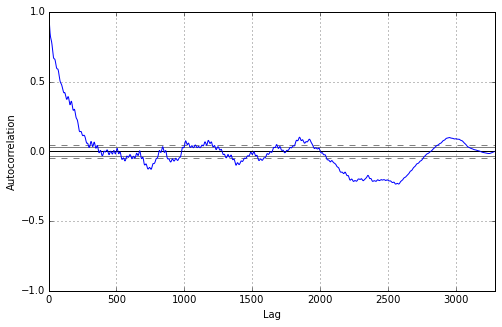
\includegraphics[width=0.5\textwidth]{figures/autocorrelation_plot}
	\caption{There is a significant memory for the market, as the autocorrelation of the 
number of HITS available (as reported by Amazon) lasts for approximately 7-10 days.}
	\label{fig:autocorrelation1}
\end{figure}

\subsection{New Tasks Attract New Workers}
\begin{figure}[ht]
	\centering
		
\includegraphics[width=0.5\textwidth]{figures/scattermatrix}
	\caption{Scatter matrix comparing the different parameters in the demand and supply.}
	\label{fig:scatter_matrix}
\end{figure}
\begin{figure}[ht]
	\centering
		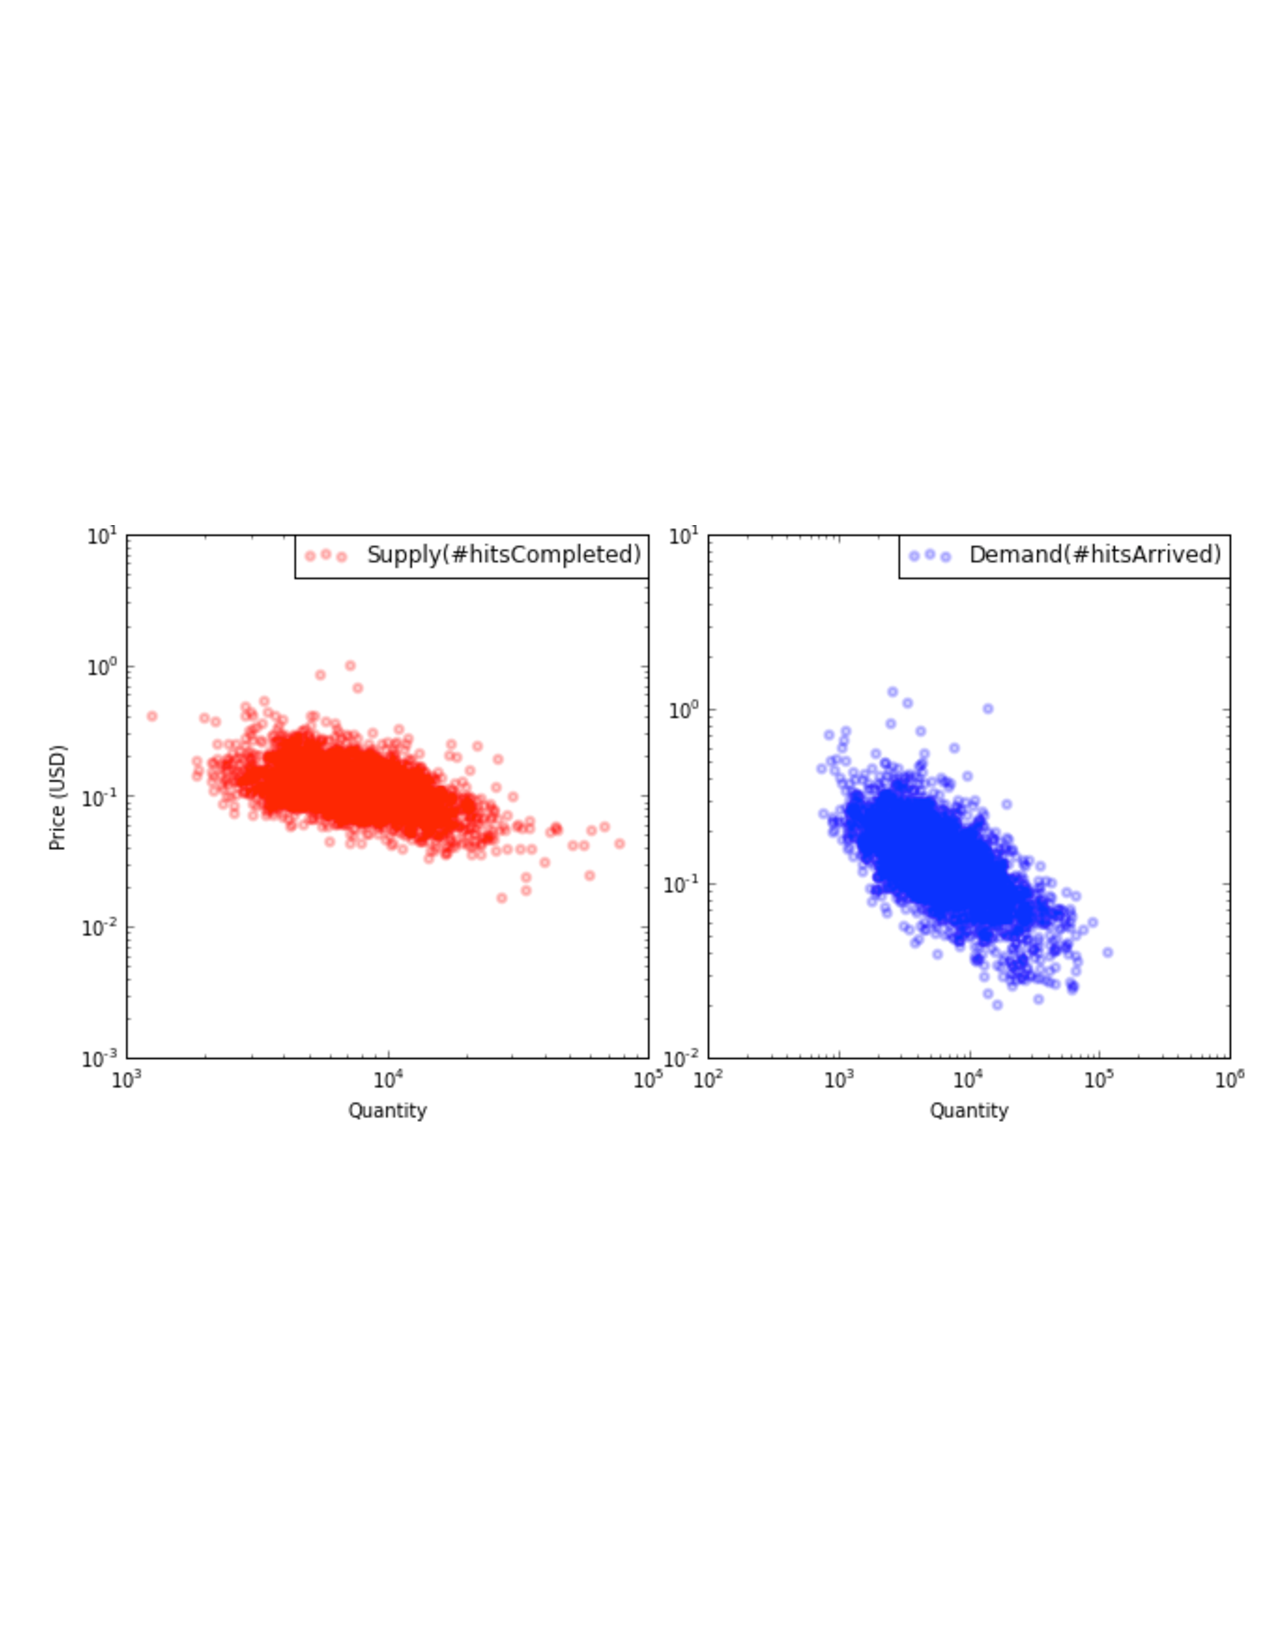
\includegraphics[width=0.5\textwidth]{figures/supply_demand}
	\caption{Demand and supply versus price.}
	\label{fig:dsup}
\end{figure}
In Figure \ref{fig:scatter_matrix} we compare  the following variables: number of HITs published on the platform, average reward of such HITs, number of HITs completed, and the average reward of such HITs. An observation  can be made about the correlation between the rewards and the number of HITs completed and those published.
The results suggest that crowd workers are sensitive to newly posted tasks, and that they are constantly monitoring for new and fresh tasks.
It must be noted that some workers may not be actively completing HITs on the platform but rather looking for HITs to work on by reading Web forums where other workers shared HITs. Thus, new HITs attract new workers to the platform.

This supplements our finding in Section \ref{sec:throughput} where we showed that $Start\_time$ is an important feature contributing to the throughput of a batch.
Figure \ref{fig:dsup}(a) shows a the expected relationship between demand and price: The larger the demand the lower the price becomes. On the other hand Figure \ref{fig:dsup}(b)  does not match the typical supply curve (higher prices drive higher supply). Instead, the demand seems to be tied to  the supply (i.e., the number of new HITs posted). A possible explanation to this effect is the lack of biding \gd{biding?} mechanisms that the workers can leverage to drive prices up.

\subsection{New Workers Complete More Tasks}
\begin{figure}[ht]
	\centering
		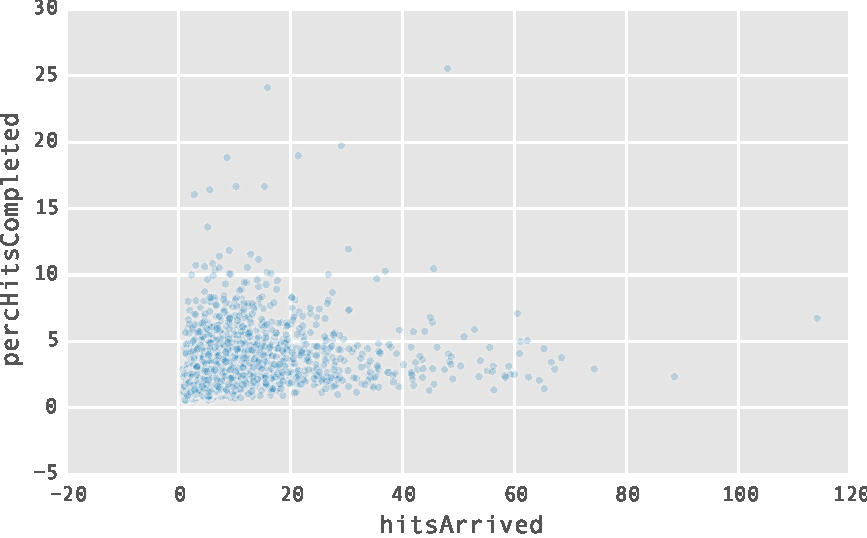
\includegraphics[width=0.5\textwidth]{figures/percHitsCompleted}
	\caption{The effect of new arrived HITs on the work  supplied.}
	\label{fig:perc_hits_completed}
\end{figure}
Along the same lines, the results detailed in Figure \ref{fig:perc_hits_completed} indicate that as more HITs are published on the platform, a higher percentage of the available work gets done. 
This clearly indicates that the arrival of new work also attracts new workers
to the market, who also seem to spillover to other tasks (i.e., not just working on the fresh HITs).

\subsection{Weekly Periodicity}
Finally, we computed the weekly moving average convergence/divergence (MACD) which is shown in Figure \ref{fig:mac}. We then run an autocorrelation to check whether there is some seasonality in the time series. Figure \ref{fig:autocorrelation2} shows that there is a strong weekly seasonality effect.
\begin{figure}[ht]
	\centering
		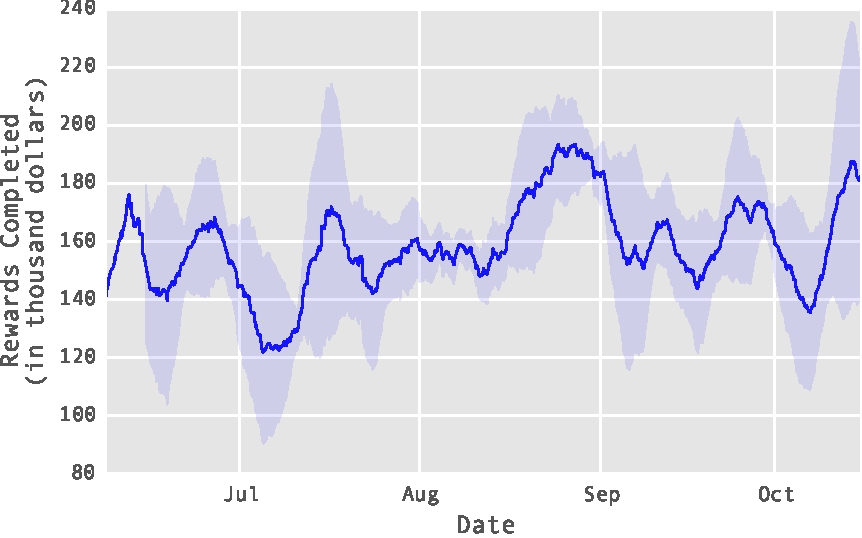
\includegraphics[width=0.5\textwidth]{figures/mac}
	\caption{Weekly Moving Average Convergence/Divergence (MACD) of the rewards for completed HITs.}
	\label{fig:mac}
\end{figure}
\begin{figure}[ht]
	\centering
		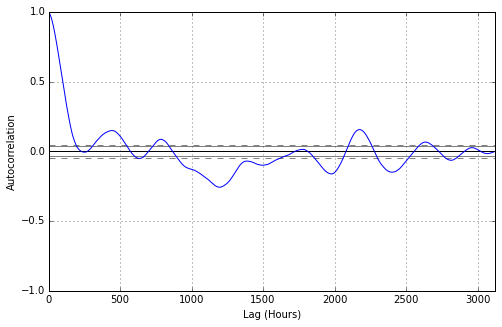
\includegraphics[width=0.5\textwidth]{figures/autocorrelation2}
	\caption{Autocorrelation computed on the weekly MACD.}
	\label{fig:autocorrelation2}
\end{figure}